\section{Exact massive vacuum reduction and retrained seed choices}
\label{sec:vac-ml}
The two-point reduction can also close when the tree ends at a massive vacuum line. We add this identity to cover connected vacuum integrals with one massive root denominator and massless bubble branches. Each branch changes the power of the root momentum, and a beta integral then evaluates the root. Appendix~\ref{app:vac-ml} defines the family and derives its rational coefficient relative to the unit-power master. This calculation uses the same subintegral principle as parametric massless reduction~\cite{Ruijl2017Forcer}, with the massive root derived explicitly here. The application checks the momenta, masses, and index powers before applying the identity, applies the rule within independent loop blocks when present, and retains the existing exact rules and Kira choices for other inputs.

For integrals that still require Kira, we train a new model to choose the sparse seed boundary before equation generation. Kira already supplies optimized seeding and equation selection~\cite{Kira3}; the learned decision chooses among three boundaries in the existing exact reduction interface. The wider and tighter boundaries come from the preceding implementation, and a third boundary gives an intermediate seed region. Appendix~\ref{app:vac-ml} derives the training objective. The seed-boundary parameters use the definition in Appendix~\ref{app:sparse}:
\begin{equation}
 \begin{split}
 \boldsymbol\theta_{\mathrm{wide}}&=(2.5,0,0,1.25,0,1,-0.25),\\
 \boldsymbol\theta_{\mathrm{tight}}&=(1,0,0,0,1,1,0),\\
 \boldsymbol\theta_{\mathrm{middle}}&=(1.5,0,0,0.5,0,1,0).
 \end{split}
 \label{eq:vac-ml-choices}
\end{equation}
These are specified candidate settings rather than physical identities. All candidates use the same protected master basis, native truncation setting, exact checks, and recovery mechanism.

The model uses 25 input features. They describe loop and external-momentum counts, propagator incidence, target count, numerator ranks, positive powers, and distances between target index vectors. The added features describe the minimum, maximum, and mean power of each of the two auxiliary denominators and the fraction of targets with zero power in each. No family name or known reduction coefficient enters the prediction. We collect complete timings for 32 training requests and 16 validation requests from planar and nonplanar massless two-loop boxes, whose propagators are defined in Appendix~\ref{app:families-new}. Their numerator ranks range from one to four, and all seven physical denominators have unit power. Each batch contains one to four targets. The sets of numerator-power pairs that define the batches are disjoint across training, validation, and the 32 reserved native requests; individual pairs can occur in different batches. Each split also uses different rational kinematics. These are new target batches within two known topology classes, so they do not establish transfer to unseen graph classes. The eligibility gate checks counts, masses, powers, and feature ranges; it does not certify that an arbitrary graph belongs to the training classes. Native basis checks and recovery retain responsibility for algebraic completion.

Candidate models contain one cost tree or an ensemble of 24 trees, using tree and bootstrap-ensemble methods~\cite{CART1984,Breiman2001Forest} with the time objective derived here. Each ensemble tree draws 32 training requests with replacement and considers a random set of 12 of the 25 features at each split. Leaves store the mean measured cost of each action, and the ensemble averages these costs. Validation compares depths one through four, minimum leaf sizes two, four, or eight, and predicted-saving margins of zero, three, eight, or fifteen percent. We enable the selected policy only if it changes at least one validation choice, adds no unverified result, and improves the fixed validation cost by at least one percent after the prediction allowance.

Validation selects 24 tree(s), maximum depth 3, minimum leaf size 2, and predicted-saving margin 0\%. The fixed comparison uses the tighter boundary, which has the lowest total validation time. The learned policy is enabled by the validation criterion. Its selected validation cost, including a two-millisecond prediction allowance per request, is 71.673 seconds, compared with 76.165 seconds for the fixed choice. These validation values select the policy and do not serve as its independent result.

We freeze the policy and implementation before testing. The exact test contains 34 distinct rooted vacuum structures, with seven targets each and a symbolic mass scale, covering every loop order from one through thirteen. Eight additional requests check the retained two-point and triangle rules. Each reserved request runs three times in fresh processes, with method order rotated and an eighteen-second application limit. The timer includes process loading, input, recognition, model loading and inference when used, native algebra and recovery, output, and exit. Direct analytic requests defer native and model imports until they are needed. Independent comparisons of returned coefficients run outside both timers. Native comparisons use the same previously verified master-index information; reference preparation is excluded equally. The previous-method comparison launches the preceding published application directly. We draw 2,000 resamples of matched requests with replacement, retain each request's paired medians, and take the 2.5 and 97.5 percentiles of the time ratios. These intervals describe variation within the finite request collection.

The new rule completes 34 of 34 vacuum requests in every repetition, while the preceding application completes 4. The reserved vacuum coefficients pass 714 independent Gamma evaluations at 80-digit precision, with scaled error below $10^{-60}$. The scaled error is the absolute difference divided by the larger of one and the reference magnitude. Separate development checks supply 9 exact coefficient comparisons with native Kira.

Before the reserved comparison, six transformation checks preserve the coefficients under loop renaming, common momentum-sign reversal, and physical-denominator reordering. Three product checks verify the integrated rule on independent vacuum blocks with four, eight, and thirteen total loops. These product checks establish composition of the supported identity and supply no separate timing claim.

\begin{table}[!htbp]\centering\small
\caption{Sums of three-run median complete times. Times use requests completed and verified by both methods. Completion counts retain all requests and require all repetitions to pass.}
\label{tab:vac-ml}
\begin{tabularx}{\linewidth}{@{}Yrrrr@{}}\toprule
Comparison & Control/new complete & Paired & Control (s) & New (s)\\\midrule
Vacuum trees versus previous & 4/34 & 4 & 5.046 & 0.730 \\
Native application versus previous & 31/32 & 31 & 186.074 & 139.678 \\
Native model versus fixed & 32/32 & 32 & 156.383 & 150.663 \\
Two-point regression checks & 4/4 & 4 & 0.626 & 0.686 \\
Triangle regression checks & 4/4 & 4 & 0.648 & 0.792 \\
\bottomrule\end{tabularx}\end{table}

The matched vacuum comparison gives time ratio 0.145, with a central 95\% request-resampling interval of $[0.096,0.379]$. The new method takes longer on 0 of the 4 matched requests.

The revised native application against the preceding application gives time ratio 0.751, with a central 95\% request-resampling interval of $[0.675,0.841]$. The new method takes longer on 10 of the 31 matched requests.

The new native model against fixed choices gives time ratio 0.963, with a central 95\% request-resampling interval of $[0.937,0.984]$. The new method takes longer on 10 of the 32 matched requests.

The final-repetition audit of the 32 matched native requests records 2 unsuccessful internal attempts with the learned choices and 14 with the fixed choice. The corresponding sums of logged equation-generation counts are 286,531 and 326,825; these count regenerated rows as further equation instances. Thus the audit distinguishes failed internal attempts that later recover from requests that never complete. The complete-time comparison includes both kinds of cost.

For the planar boxes alone, the learned-to-fixed ratio is 0.929, with request interval $[0.870,0.977]$ on 16 matched requests. For the nonplanar boxes alone, the learned-to-fixed ratio is 0.978, with request interval $[0.952,0.997]$ on 16 matched requests.

The new model runs on 26 of the 32 reserved native requests. The application retains the selected fixed choice outside the training feature ranges. The ML comparison holds the exact identities and native machinery fixed, while the vacuum comparison measures the new analytic identity. We do not assign finite speed factors to failed controls or combine gains from different experiments by multiplication. These results extend the exact domain to the specified single-mass vacuum trees and test native learned choices on the stated two-loop boxes. General massive scattering, unrestricted numerators, and arbitrary high-loop graphs remain outside this demonstrated coverage.

\subsection{Final application test with the trained policy fixed}
The preceding comparison showed that application overhead can matter when the exact coefficient takes little time to compute. We therefore reduce repeated output bookkeeping and keep the formulas, trained weights, seed choices, and recovery unchanged. We then freeze this revision before a separate test on 22 fresh requests. Fourteen requests use the exact rules: twelve chain requests cover vacuum, two-point, and triangle roots at one, three, seven, and thirteen loops, while two branched thirteen-loop requests each contain 128 targets. Eight native requests use new numerator-batch sets in the same two box classes. These sets occur in neither fitting nor the preceding reserved comparison. The rational native kinematics also change. Each request runs three times in a fresh process with the same complete-time convention and exact checks.

\begin{table}[!htbp]\centering\small
\caption{Separate test of the final application. Each row sums request medians over matched completed requests. The fixed control disables the new model in the final application. These results use a new collection and do not replace the preceding comparison.}
\label{tab:vac-ml-final}
\begin{tabularx}{\linewidth}{@{}Yrrr@{}}\toprule
Comparison & Paired & Control (s) & Final (s)\\\midrule
Exact rules versus first revision & 14 & 2.994 & 2.756 \\
Native application versus first revision & 8 & 62.057 & 59.963 \\
Retained exact rules versus preceding method & 9 & 1.769 & 1.863 \\
Native model versus fixed choice & 7 & 45.471 & 43.792 \\
\bottomrule\end{tabularx}\end{table}

The final application completes 22 of the 22 requests in every repetition. On the eight native requests, the learned application completes all eight in every repetition, while the fixed control completes 7 in every repetition. Its time ratio therefore uses 7 paired requests; the incomplete control receives no finite speed factor. The exact-output comparisons verify 4821 coefficients across the timed methods and repetitions. All final requests relative to the first revision give time ratio 0.964, with request interval $[0.925,0.997]$. The retained exact requests relative to the preceding method give time ratio 1.053, with request interval $[0.977,1.138]$. This interval includes equal time. The unchanged native model relative to the final fixed choice give time ratio 0.963, with request interval $[0.899,0.999]$. The two native test collections remain separate: the final test checks the deployed application with unchanged weights, and supplies no further model selection. Short analytic requests can still take longer than the preceding specialized application because recognition and dispatch have a cost.

\begin{figure}[!htbp]\centering
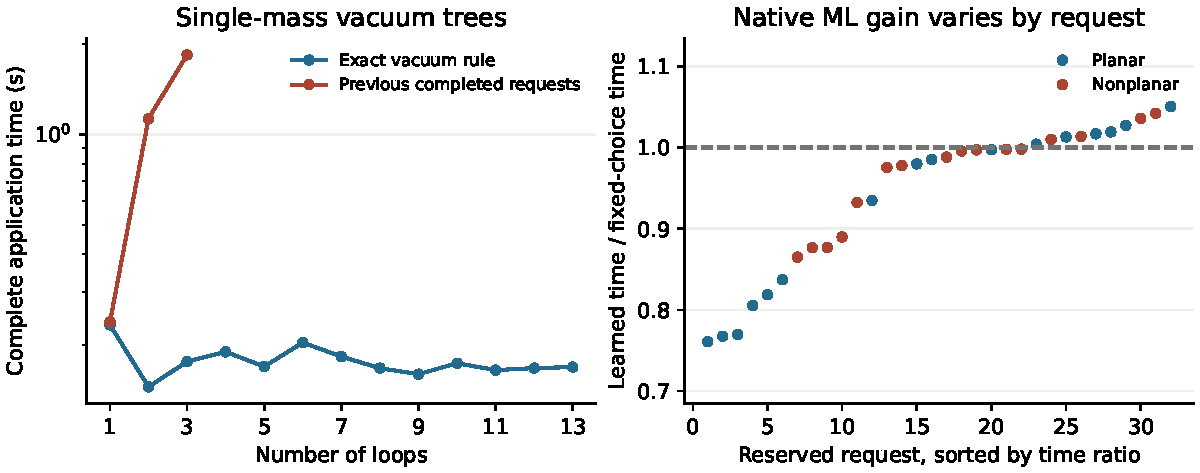
\includegraphics[width=\linewidth]{paper_figures/vacuum_learning.pdf}
\caption{The left panel shows mean request medians at each loop order for the vacuum trees; absent control points indicate that no control completed at that order. The right panel shows each matched native request relative to the fixed validation-selected seed setting. Ratios below one indicate less complete time. The equal-time line makes regressions visible.}
\label{fig:vac-ml}
\end{figure}
\FloatBarrier
